\chapter{Bibliotheken und Assets}

\section{Into The Sky}

Aufgrund der notwendigen geringen Latenz ist es bei MMOFPS-Spielen empfehlenswert, ein Binärformat zur Serialisierung von Datenstrukturen zu verwenden. Für Into The Sky habe ich mich daher für die Verwendung von Protobuf entschieden.

Im Vergleich zu neueren Verfahren wie Cap'n Proto ist deutlich mehr Dokumentation vorhanden, was die Arbeit an dem Projekt beschleunigt. Im Gegensatz zu Formaten wie JSON ist Protobuf im Hinblick auf die Datenpakete deutlich effizienter. Die Verwendung eines kompakten Binärformats verringert die zu übertragene Datenmenge erheblich. Der Nachteil von Strukturierten Formaten wie JSON ist, dass Daten wie Feldnamen oder Klassennamen mit übertragen werden. Das macht die Daten zwar leichter wartbar, in diesem Kontext ist allerdings die Effizienz von höchster Priorität.

Der Ansatz, der zu Beginn der Implementierung vorgelegen hat, basiert auf Reflection. Protobuf ist als etabliertes Verfahren jedoch vorzuziehen und bietet diverse Optimierungen, die durch einen Eigenbau nicht erreicht werden können. In der Präsentation zu diesem Thema habe ich ursprünglich vorgeschlagen Netcode for Game Objects zu verwenden. Diese Bibliothek ist jedoch nicht mit den Architekturvorschlägen und den ersten Umsetzungen kompatibel.

\subsection{Entwicklung des Proof-of-Concept}

Der Prozess, um ein Proof-of-Concept zu realisieren, ist einfach und geradlinig. Als erstes wird ein  neues Projekt in Visual Studio angelegt. Dabei handelt es sich um eine Class Library. Der Unity-Version ist zu entnehmen, dass die Objekte den .NET Standard 2.1 unterstützen. Diese Zielversion wird auch für die Class Library verwendet. Über NuGet wird Protobuf installiert, dabei ist die aktuellste Version benutzbar (zum aktuellen Zeitpunkt 3.26.1). Anschließend wird die Struktur der Netzwerkbibliothek angelegt.

\begin{figure}[!h]
	\centering
	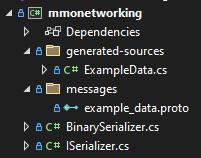
\includegraphics[width=6cm]{figures/networkingstructure.png}
	\caption{Struktur der Netzwerkbibliothek}
	\label{fig:networkingstructure}
\end{figure}

Der Ordner \verb|generated-sources| wird zunächst leer gelassen. Dort landen die generierten C\#-Dateien von Protobuf. Um die Dateien zu erstellen muss zunächst \verb|protoc| installiert werden. Anschließend muss das Bauen der Protobuf Dateien in den Build-Prozess von Visual Studio eingebunden werden. Dies geschieht, indem man den folgenden Befehl als Build-Event einfügt:

\begin{quote}
	\centering
	protoc -I=\verb|"|\$(ProjectDir)messages\verb|"| --csharp\_out=\verb|"|\$(ProjectDir)generated-sources\verb|"| \verb|"|\$(ProjectDir)messages\*.proto\verb|"|
\end{quote}

\begin{figure}[!h]
	\centering
	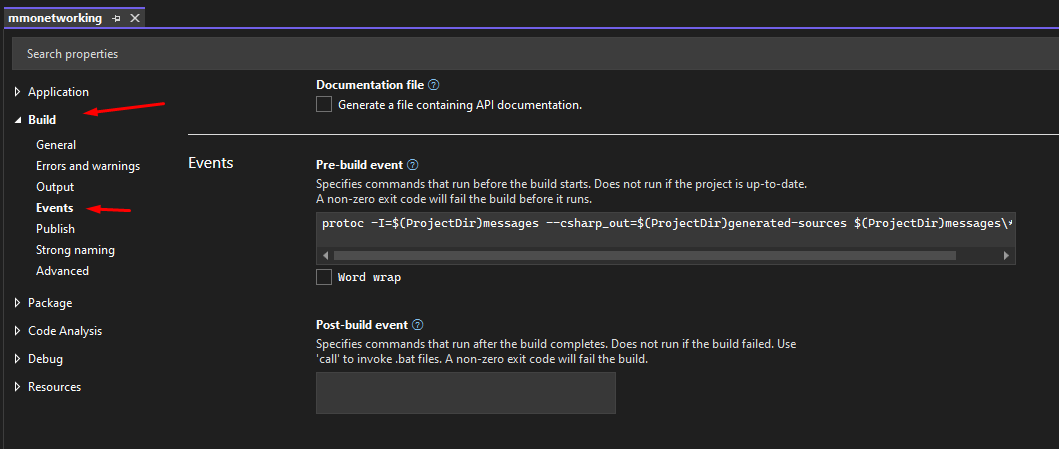
\includegraphics[width=16cm]{figures/networkingprotobuild.png}
	\caption{Build-Befehl}
	\label{fig:networkingbuildcommand}
\end{figure}

Dieser Befehl kompiliert die Proto-Dateien im messages Ordner und erzeugt die C\# Quelldateien im generated-sources Ordner. Durch das Build-Event wird dies vor jeder Kompilierphase durchgeführt.

Nach dem Erstellen einer Muster-Datei zur Datenübertragung die einige Beispielfelder enthält, wird diese zu einer C\#-Datei kompiliert. Nun kann ein einfacher Serialiser geschrieben werden, der die von Protobuf bereitgestellten Methoden nutzt. Im Anschluss kann das Projekt mit \verb|Build -> Build Solution| gebaut werden. Im Output ist nun erkennbar wo sich die gebaute DLL befindet. Neben dieser DLL müssen die DLL's von Protobuf und einer Abhängigkeit von Protobuf (System.Runtime.CompilerServices.Unsafe) heruntergeladen oder aus dem System entnommen werden. Dabei wird die Version 6.0.0 der Abhängigkeit benötigt.

Diese Abhängigkeiten werden im Client-Projekt von Into The Sky eingefügt. Der Zielordner ist \verb|Assets/Plugins|. Dorthin werden die insgesamt drei DLL's Kopiert.

Der Proof-of-Concept wird durch das Erstellen eines neuen Scripts abgeschlossen. Dort kann nun der Serialiser benutzt werden. Auch die Klassen, die durch den Protobuf-Compiler erstellt wurden, sind verfügbar und können zur Serialisierung der Daten benutzt werden. Dies ist im aktuellen Projektstand in einer eigenen Szene \verb|"|SerializationTestScene\verb|"| im \verb|"|Serialization-SanityChecker\verb|"|-Skript testweise realisiert. 


\subsection{Tests}

Um die Serialisierung zu testen, habe ich ein zweites Projekt der Solution hinzugefügt. Dieses wird als \verb|MSTest Test Project| erstellt und bringt die nötigen Mittel mit, um eine Class Library zu testen. Nachdem die Class Library als Abhängigkeit eingetragen wurde kann man nun Unit-Test-Klassen schreiben. In diesem Fall habe ich folgende Testfälle initial angelegt, diese werden vermutlich im Laufe des Projekts erweitert. Die Tests werden nach einer stets gleichen Struktur benannt: Zuerst wird die Situation beschrieben, anschließend die Eingabe die getestet werden soll und zuletzt das zu erwartende Ergebnis notiert.

\begin{figure}[!h]
	\centering
	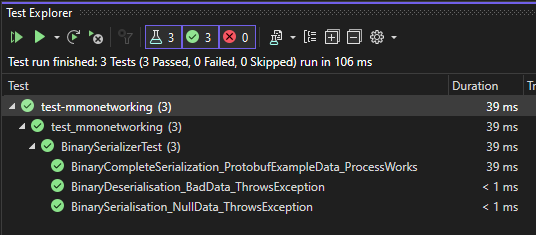
\includegraphics[width=16cm]{figures/intotheskytests.png}
	\caption{Beispielhafte Test-Cases (Into The Sky)}
	\label{fig:networkingstructure}
\end{figure}

\section{Park Chase}

Für Park Chase habe ich mich für einen einfachen JSON-Serialiser entschieden. Übertragungsgeschwindigkeit und Latenz sind aufgrund des Spielkonzepts von Park Chase weniger kritisch. Außerdem wird das Spiel auf verschiedensten mobilen Endgeräten gespielt werden. Um dort vergleichsweise einfach das Spiel zu testen ist es wichtig, lesbare Formate zu benutzen. In diesem Fall habe ich mich für JSON aufgrund seiner einfachen Struktur und direkten Unterstützung durch Unity entschieden.

\subsection{Entwicklung der Serialisierungs-Klasse}

Unity enthält bereits eine Klasse, welche die JSON Serialisierung durchführt. Dabei handelt es sich um die Klasse \verb|JsonUtility|. Diese eigene Klasse beinhaltet im wesentlichen nur Aufrufe der Methoden vom  \verb|JsonUtility| und dem Umwandeln des JSON-Strings in ein UTF-8 kodiertes Byte-Array.

\subsection{Tests}

Die Testfälle zu dieser Klasse sind ähnlich zu dem der Tests von Into The Sky aufgebaut. Hier werden allerdings die Test-Strukturen von Unity direkt verwendet. 

\begin{figure}[!h]
	\centering
	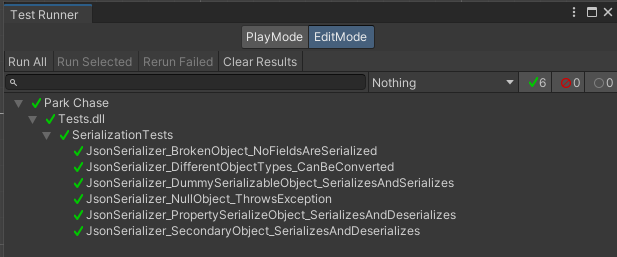
\includegraphics[width=16cm]{figures/parkchasetests.png}
	\caption{Beispielhafte Test-Cases (Park Chase)}
	\label{fig:parkchasetests}
\end{figure}

Die Test-Strukturen erlauben es auch, Tests im laufenden Spielbetrieb laufen zu lassen. Dies ist für diese Klasse jedoch nicht sinnhaft, weshalb ein Unit-Test vollkommen ausreichend ist.

\newpage

